\section{Lógica de las Data Classes}

Para la correcta interpretación y manipulación de la información intercambiada entre la aplicación móvil y los servidores (tanto el de Spring Boot como el de la Red Neuronal), el sistema hace uso de Data Classes de Kotlin. Estas clases son un componente esencial en la arquitectura de datos del proyecto, ubicadas principalmente en el paquete `com.example.prueba3.DataClasses`.

\subsection{Propósito y Características de las Data Classes}

Las Data Classes en Kotlin están específicamente diseñadas para contener datos. El compilador de Kotlin genera automáticamente funciones útiles para ellas, como `equals()`, `hashCode()`, `toString()`, `copy()`, y `componentN()`, lo que las hace ideales para modelar la estructura de los datos que se reciben de las APIs o se envían a ellas.

Su rol principal en el sistema es:
\begin{itemize}
	\item \textbf{Modelado de Estructuras de Datos:} Definen de forma clara y concisa la estructura de los objetos JSON que se serializan o deserializan a través de Retrofit y Gson. Cada propiedad de una Data Class se mapea a un campo correspondiente en el JSON.
	\item \textbf{Inmutabilidad y Seguridad:} Por convención, las propiedades de las Data Classes se declaran como `val` (valores inmutables), lo que promueve una gestión de datos más segura y predecible a lo largo de la aplicación.
	\item \textbf{Facilidad de Uso con Retrofit y Gson:} Son perfectamente compatibles con `GsonConverterFactory` de Retrofit, lo que permite que el proceso de conversión de JSON a objetos Kotlin y viceversa sea automático y eficiente.
\end{itemize}

\subsection{Ejemplos de Data Classes Implementadas}

A continuación, se presentan ejemplos de Data Classes utilizadas en el proyecto para ilustrar su función en el modelado de la información:

\begin{figure}[H]
	\centering
	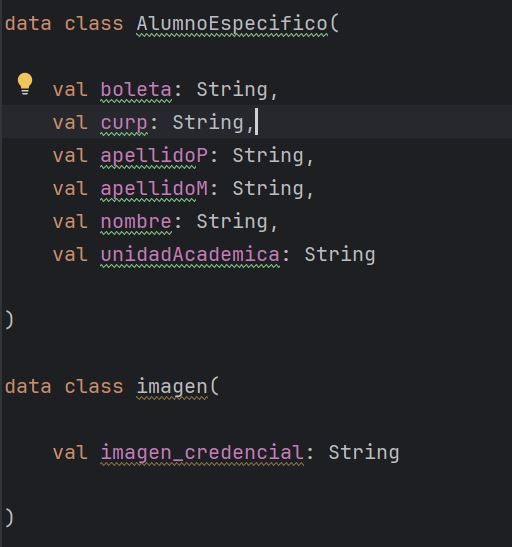
\includegraphics[width=0.7\textwidth]{ImagenesDetalles/clase.jpg}
	\caption{Entidad Usuario dentro del servidor.}
	\label{fig:Detalle clases}
\end{figure}

Estas Data Classes, junto con otras implementadas en el proyecto, aseguran que los datos sean manejados de manera estructurada y segura a lo largo de la aplicación móvil, facilitando la comunicación con los servicios backend y la manipulación de la lógica de negocio.